\documentclass[12pt]{beamer}
\usetheme{default} 

\setbeamertemplate{navigation symbols}{} %gets rid of navigation symbols
\setbeamertemplate{footline}{} %gets rid of bottom navigation bars
\setbeamertemplate{footline}[page number]{} %use this for page numbers

\setbeamertemplate{footline}{%
  \raisebox{5pt}{\makebox[\paperwidth]{\hfill\makebox[10pt]{\scriptsize\insertframenumber~~}}}}

\setbeamertemplate{itemize items}[circle] %round bullet points
\setlength\parskip{10pt} % white space between paragraphs

\usepackage{wrapfig}
\usepackage{subfig}
\usepackage{setspace}
\usepackage{enumerate}
\usepackage{graphicx}
\usepackage{amsmath}
\usepackage{amsfonts}
\usepackage{amssymb}
\usepackage{amsthm}
\usepackage[UKenglish]{isodate}
\usepackage{tikz}
\usepackage{pgfplots}
\usepackage{natbib}
\usepackage{hyperref}
\hypersetup{
    colorlinks=true, 
    urlcolor=blue
}
\def\checkmark{\tikz\fill[scale=0.4](0,.35) -- (.25,0) -- (1,.7) -- (.25,.15) -- cycle;} 

% allow drawing arrows
\usetikzlibrary{arrows}
\tikzstyle{arrow}=[draw, -latex] 

% bracketing shortcuts
\newcommand{\paren}[1]{\left(#1\right)}
\newcommand{\sqbracket}[1]{\left[#1\right]}
\newcommand{\cbracket}[1]{\left\{#1\right\}}
\newcommand{\abs}[1]{\left\lvert#1\right\rvert}
\newcommand{\norm}[1]{\left\lVert#1\right\rVert}
% set up the argmin operator, argmax
\DeclareMathOperator*{\argmin}{arg\,min}
\DeclareMathOperator*{\argmax}{arg\,max}

\newcommand{\myframe}[1]{\begin{frame} \frametitle{#1}}
% the preamble
\title{Day 1, Session 1: Overview}
\author{Gillian Tarr and Brian D. Williamson}
\institute{EPI/BIOST Bootcamp 2016}
\date{23 September 2016}

% Start the document
\begin{document}
% The title page
\begin{frame}
\titlepage
\end{frame}

\myframe{Welcome!}
\begin{itemize}
\item Welcome to the first EPI/BIOST Bootcamp!
\item[]
\item For today:
\begin{itemize}
\item Our backgrounds
\item[]
\item Introduction to course content for EPI 511 and BIOST 511
\item[]
\item Overview of this course
\item[]
\item Some skills and resources for success in graduate school
\end{itemize}
\end{itemize}
\end{frame}

\myframe{Our backgrounds: Gillian}

\end{frame}

\myframe{Our backgrounds: Brian}
\centering
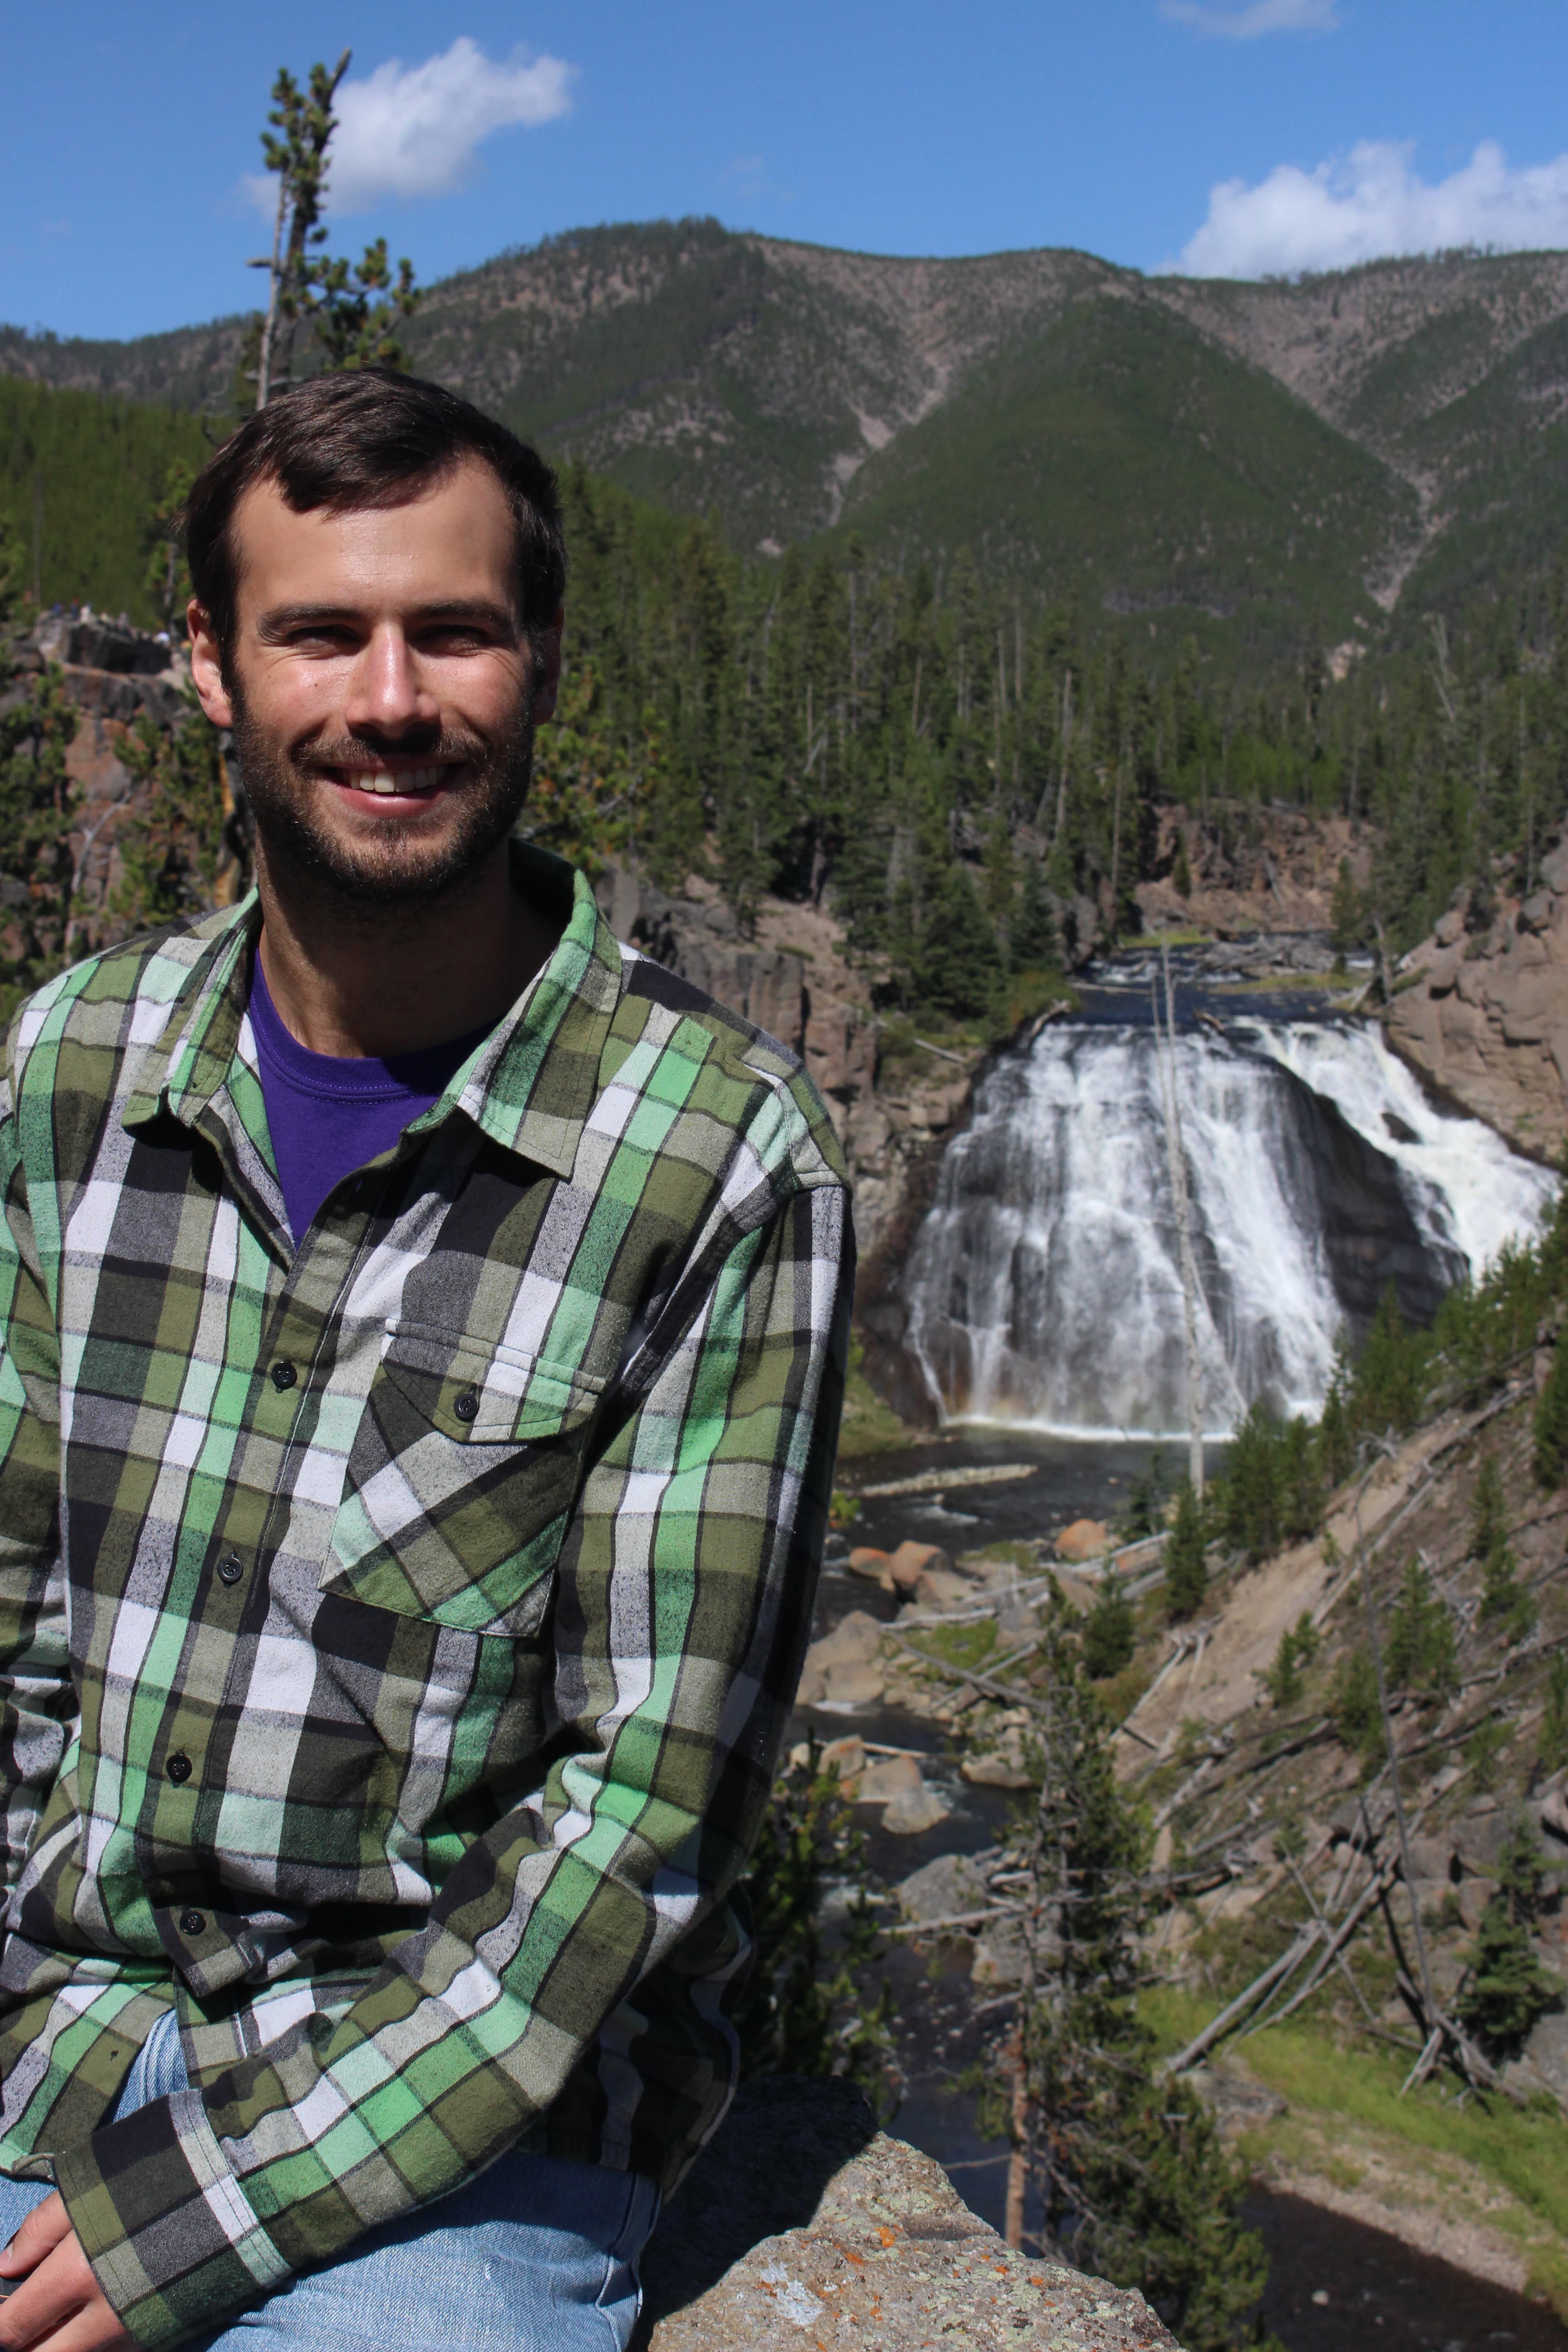
\includegraphics[width = .25\textwidth]{yellowstone-min.jpg}
\begin{itemize}
\item Third year PhD student, Biostatistics
\item[]
\item Past TA for R in BIOST 511, 512, 517, 518
\item[]
\item 
\end{itemize}
\end{frame}

\myframe{Intro to course content: EPI 511}

\end{frame}

\myframe{Intro to course content: BIOST 511}
\begin{itemize}
\item Objective: provide students with an understanding of basic concepts and methods of statistical inference in the health sciences
\item[]
\item Some major topics:
\begin{itemize}
\item Data description, exploratory data analysis
\item[]
\item Basic issues in study design
\item[]
\item Probability concepts and models
\item[]
\item Statistical inference - estimation and hypothesis testing
\item[]
\item Categorical data analysis
\item[]
\item Introduction to regression analysis
\end{itemize}
\end{itemize}
\end{frame}

\myframe{Intro to course content: BIOST 511}
\begin{itemize}
\item Only pre-requisite is basic algebra
\item[]
\item However, R will be used to teach some of the concepts and analyze data
\item[]
\item 
\end{itemize}
\end{frame}

\myframe{Overview of the bootcamp}
\begin{itemize}
\item Today: overview, etc
\item[]
\item 26 September: Algebra and more!
\begin{itemize}
\item Order of operations and negative numbers
\item[]
\item Fractions
\item[]
\item Algebra
\item[]
\item Graphs
\item[]
\item Logs and exponents
\item[]
\item Word problems etc
\end{itemize}
\end{itemize}
\end{frame}

\myframe{Overview of the bootcamp}
\begin{itemize}
\item 27 September: R!
\begin{itemize}
\item Using scripts, the console, and simple tasks
\item[]
\item Installing and loading packages. Case study: \texttt{uwIntroStats}
\item[]
\item Data types, data structures
\item[]
\item Loading data and running scripts
\end{itemize}
\end{itemize}
\end{frame}

\myframe{Skills for success}

\end{frame}

\myframe{Exercises for the weekend}
\begin{itemize}
\item Visit the R project page at \url{https://cran.r-project.org/} and download R
\item[]
\item Visit the RStudio page at \url{https://www.rstudio.com/} and download RStudio
\item[]
\item Visit the GitHub page for this bootcamp at \url{https://github.com/UW-EPI-BIOST-PREP/Epi-Biost-Workshop2016}
\begin{itemize}
\item Download the slides and other materials using the green ``Clone or Download'' button (choose download)
\end{itemize}
\item[]
\end{itemize}
\end{frame}

\myframe{Exercises for the weekend}
\begin{itemize}
\item Visit the \texttt{uwIntroStats} page at \url{http://uwintrostats.org/index.asp} and download the package
\item[]
\item If you have trouble with any of the steps (besides GitHub), there are help videos on the uwIntroStats website
\item[]
\end{itemize}
\end{frame}

\myframe{Exercises for the weekend}
\begin{itemize}
\item Install the \texttt{uwIntroStats} package:
\begin{enumerate}
\item Open RStudio once it and R are installed
\item[]
\item Go to the ``Tools'' menu, and select ``Install Packages...''
\item[]
\item In the dropdown menu for ``Install from:'', select ``Package Archive File (.zip, .tar.gz)''
\item[]
\item Navigate to where \texttt{uwIntroStats} downloaded and select the package file
\item[]
\item Click ``Install'' if necessary
\end{enumerate}
\end{itemize}
\end{frame}
\end{document}